%&pdflatex
\documentclass{article}
\usepackage[final]{nips_2017}
\usepackage[utf8]{inputenc} % allow utf-8 input
\usepackage[T1]{fontenc}    % use 8-bit T1 fonts
\usepackage{hyperref}       % hyperlinks
\usepackage{url}            % simple URL typesetting
\usepackage{booktabs}       % professional-quality tables
\usepackage{amsfonts}       % blackboard math symbols
\usepackage{nicefrac}       % compact symbols for 1/2, etc.
\usepackage{microtype}      % microtypography
\usepackage{amsmath}
\usepackage{mathtools}
\usepackage{graphicx}
\usepackage{tabu}
\usepackage{mathrsfs}
\usepackage{morefloats}
\usepackage{float}
\usepackage{listings}
\usepackage[usenames,dvipsnames]{xcolor}
\usepackage{commath}
\usepackage{graphicx}
\usepackage{tikz,tikz-3dplot}
\usepackage{longtable}
\usetikzlibrary{calc}
\usetikzlibrary{intersections}

% Define the coloring for keywords in Julia
\lstdefinelanguage{Julia}%
{morekeywords={abstract,break,case,catch,const,continue,do,else,elseif,%
    end,export,false,for,function,immutable,import,importall,if,in,%
    macro,module,otherwise,quote,return,switch,true,try,type,typealias,%
    using,while},%
  sensitive=true,%
  morecomment=[l]\#,%
  morecomment=[n]{\#=}{=\#},%
  morestring=[s]{"}{"},%
  morestring=[m]{'}{'},%
}[keywords,comments,strings]%

% Set the lstlistings to the Julia color scheme
\lstset{
  basicstyle       = \ttfamily,
  columns          = fullflexible,
  frame            = none,
  breaklines       = true,
  language         = Julia,
  basicstyle       = \ttfamily,
  keywordstyle     = \bfseries\color{blue},
  stringstyle      = \color{magenta},
  commentstyle     = \color{ForestGreen},
  showstringspaces = false,
  numbers          = left,
  xleftmargin      = 2em,
  framexleftmargin = 2em
}

\title{Scale Space Edge Detection}

\author{
  Nicholas Draper, Jonathan Hayase\\
  Seminar in Differential Geometry\\
  Harvey Mudd College
}

\begin{document}
\maketitle

\begin{abstract}
  Scale space representation of an image is the idea that a two dimensional image can be represented by a collection of smoothed images.
  This paper documents how using such a representation can be useful for detecting edges in an image.
  In addition to the theory, this paper also covers an in depth implementation of the algorithm written in the Julia programming language.
\end{abstract}

\section{Introduction}
Detecting edges in images has long been a persistent problem in image processing.  
Generally speaking, the majority of algorithms usually detect edges by identifying at least one of the following features:
\begin{itemize}
\item large discontinuities in luminance values
\item discontinuities in different object orientations
\item large discontinuities in the intensity gradient
\end{itemize}
In this paper, we will be using the scale space representation of an image to approach the edge detection problem.
Scale refers to how much smoothing is applied to the image. 
The theory behind the scale space representation is that detecting one-dimensional image features, like edges, may be dependent on what scale we operate at \cite{Lindeberg1998}. 
It follows that we can then define a scale space edge as a set of connected points that:
\begin{itemize}
\item have a gradient that assumes a local maximum value in the direction of the gradient\cite{Lindeberg1998}
\item have an edge strength metric which is a local maximum over various scales\cite{Lindeberg1998}.
\end{itemize}

\section{Motivation}
The motivation for this paper comes from observing how much the scale affects the detection of edges in an image. 
Most common edge detection algorithms are applied only at a scale of zero, i.e. the original image.
Common methods for detecting edges in images usually consist of convolving a discrete derivative matrix with the image to calculate spatial derivatives of the image.
Algorithms like the Sobel, Canny, Roberts, and Prewitt do just exactly that. 
The problem with these methods is that they are not very adaptable, and they could be possibly neglecting useful information at other scales. 
For example, given an image ${F}$, the following computes the gradient of the image in the $x$ and $y$ direction using the Sobel operator
\begin{equation}
	{G}_x =
	\begin{bmatrix}
		+1 &0 &-1 \\
		+2 &0 &-2 \\
		+1 &0 &-1 
	\end{bmatrix}
	* {F}, \;
	{G}_y =
	\begin{bmatrix}
		+1 &+2 &+1 \\
		0 &0 &0 \\
		-1 &-2 &-1 
	\end{bmatrix}
	* {F}
\end{equation}
Our algorithm will consist of convolving the ando5 matrix, which is more rotationally symmetric than the other operators listed above, with the image. 
This convolution will be be performed at multiple scales to evaluate the criteria necessary for classifying a point as an edge point in the scale space. 
We then run a marching cubes algorithm to connect the local maxima and list our edges based on strength. 
The ability to list edges and classify their strengths is one of the advantages that the scale space edge algorithm has over conventional methods. 

\section{Scale Space and Its Derivatives}
To understand how exactly we detect edges in the scale space, we must first define what the scale space is.
If we have a continuous function of multiple variables such as $f(x,y)$, then we define the scale space representation of such a function as the following convolution
\begin{equation}
  L(x,y;t) = g(x,y;t) * f(x,y)
\end{equation}
Here $t$ represents the scale parameter, and can be thought of how much smoothing is applied to the function. The function $g$ is the Gaussian kernel given by
\begin{equation}
  g(x,y;t) = \frac{1}{2 \pi t}e^{-(x^2+y^2)/(2t)}
\end{equation}
With the scale space representation defined, we can now take derivatives of it as it is a continuous well-defined function.
Spatial derivatives are relatively simple being defined as the following
\begin{equation}
  L_{x^{\alpha}y^{\beta}}(\cdot;t) = \partial_{x^{\alpha}y^{\beta}}L(\cdot;t) = g_{x^{\alpha}y^{\beta}}(\cdot;t) * f(\cdot)
\end{equation}
However, when taking the partial derivative with respect to the scale $t$, it becomes more interesting.
The scale space representation collection is a solution for the diffusion equation. Therefore is has the useful property of \cite{Lindeberg1993}
\begin{equation}
  \partial_t L = \frac{1}{2} \nabla^2 L = \frac{1}{2} (\partial_{xx} + \partial_{yy})L
\end{equation}
with the initial condition of $L(x,y;0) = f(x,y)$.
So we can now represent scale derivatives as spatial derivatives. 

Now all these representations and operators are useful for continuous functions, but the images we deal with are discrete and contain quantized intensity values.
So we must now understand how these operations and properties apply to the discrete domain.

The scale space representation is still defined in a similar fashion.
The following is the discrete version of the scale space operating on the function $f(x)$
\begin{equation}
  L(x;t) = (T(\cdot;t) * f(\cdot))(x;t)
\end{equation}
In this expression, $T$ represents the discrete version of the Gaussian kernel and is further evaluated as \cite{Lindeberg1993}
\begin{equation}
  T(n;t) = e^{-t}I_n(t)
\end{equation}
where $I_n$ is the modified Bessel functions of integer order given by
\begin{equation}
  I_n(x) = i^{-n}J_{n}(ix) = \sum_{m=0}^{\infty}\frac{1}{m!\Gamma(m+n+1)}\left(\frac{x}{2}\right)^{2m+n}
\end{equation}
Now that the one dimensional case is understood for the scale space, we can expand this to two dimensions.
After all, images are composed of two dimensions, so it makes sense that these operators can act on two dimensional functions.
The two dimensional scale space representation for discrete variables is given by the following
\begin{equation}
  L(x,y;t) = \sum_{m=-\infty}^{\infty}\sum_{n=-\infty}^{\infty}T(m;t)T(n;t)f(x-m,y-n)
\end{equation}
Even with the discrete case, the scale space representation must still satisfy the semidiscretized version of the diffusion equation.
Therefore by taking a scale derivative of the function we must have the following \cite{Lindeberg1993}
\begin{equation}
  \partial_t L = \frac{1}{2}((1-\gamma)\nabla^2_5L+\gamma\nabla^2_\times L)
\end{equation}
where $\gamma \in [0,1]$ is a hyperparameter and,
\begin{equation}
  (\nabla^2_5f)_{0,0} = f_{-1,0} + f_{+1,0} + f_{0,-1} + f_{0,+1} - 4f_{0,0}
\end{equation}
\begin{equation}
  (\nabla^2_\times f)_{0,0} = \frac{1}{2}(f_{-1,-1} + f_{-1,+1} + f_{+1,-1} + f_{+1,+1} - 4f_{0,0})
\end{equation}
Note that $f_{-1,1}$ represents $f(x-1, y+1)$. Now that we have defined what discrete scale spaces and their derivatives look like, we can start to define what an edge is.

\section{Defining an Edge in Scale Space}
A useful thing to do when dealing with image features is to set up a coordinate system in terms of the local directional derivatives.
In this case, we do the same thing as the paper does and setup a coordinate system $(u,v)$ at any point $(x_0,y_0)$ on the image.
Here, the $v$-axis is parallel to the gradient direction at the point $(x_0, y_0)$, and the $u$-axis is perpendicular to the gradient direction at the same point. So then we define necessary angles as \cite{Lindeberg1998}
\begin{equation}
  \begin{pmatrix}
    \cos{\alpha} \\
    \sin{\alpha}
  \end{pmatrix}
  = \frac{1}{\sqrt{L_x^2+L_y^2}}
  \begin{pmatrix}
    L_x \\
    L_y
  \end{pmatrix}
  \Bigg|_{(x_0,y_0)}
\end{equation}
With our angles defined, we can then define our $(u,v)$ coordinate system by taking the respective partial derivatives of our spatial coordinate system
\begin{align}
  \partial_u &= \sin{\alpha}\; \partial_x - \cos{\alpha}\; \partial_y \\
  \partial_v &= \cos{\alpha}\; \partial_x + \sin{\alpha}\; \partial_y
\end{align}
So then we can define our partials of $L$ with respect to this new $(u,v)$ coordinate system. The results for $L_v$ can be found on page \pageref{t_v}. So then we define an edge in this coordinate system with the following conditions \cite{Lindeberg1998}
\begin{equation} \label{eq:c1}
  \begin{aligned}
    L_{vv} &= 0 \\
    L_{vvv} &< 0
  \end{aligned}
\end{equation}
The way we can then represent these conditions in terms of spatial derivatives is as follows \cite{Lindeberg1998}
\begin{equation}
  \begin{aligned}
    L_{vv} &= L_x^2L_{xx}+2L_xL_yL_{xy}+L_y^2L_{yy} = 0 \\
    L_{vvv} &= L_x^3L_{xxx} +3L_x^2L_yL_{xxy}+3L_xL_y^2L_{xyy}+L_y^3L_{yyy} < 0
  \end{aligned}
\end{equation}
The results for $L_{vv}$ can be found on page \pageref{t_vv}.
The results for $L_{vvv}$ can be found on page \pageref{t_vvv}.
This is useful for determining edges at a single scale, but if we are to determine edges over multiple scales, we must also develop an edge strength metric, $\varepsilon_{norm}L$.
Thus this adds two more conditions that must be satisfied for an edge to be classified in the scale space \cite{Lindeberg1998}
\begin{equation} \label{eq:c2}
  \begin{aligned}
    \partial_t(\varepsilon_{norm}L(x,y;t)) = 0\\
    \partial_{tt}(\varepsilon_{norm}L(x,y;t)) < 0
  \end{aligned}
\end{equation}
Then (Eq. \ref{eq:c1}) in conjunction with (Eq. \ref{eq:c2}) form the necessary constraints for us to define an edge in the scale space.
Now we must define what we mean by edge strength and give a clearer idea of $\varepsilon_{norm}$.

The approach we took was to let our edge strength metric be defined by the gradient magnitude that has been normalized by our $\gamma$ factor. 
Our results for the following calculations can be found on page \pageref{t_gma}.
In this case we can define our normalized gradient magnitude as \cite{Lindeberg1998}
\begin{align}
  G_{\gamma}L &= L_{v,\gamma}^2 \\
  &= t^{\gamma}(L_x^2+L_y^2)
\end{align}

The first scale derivative of the gradient magnitude results are found on page \pageref{t_tgma}. 
Its calculations are as follows \cite{Lindeberg1998}
\begin{equation} \label{dtGl}
  \partial_t (G_{\gamma}L) = \gamma t^{\gamma-1}(L_x^2+L_y^2) + t^{\gamma}(L_x(L_{xxx}+L_{yyy})+L_y(L_{xxy} + L_{yyy}))
\end{equation}
Then the second scale derivative of the gradient magnitude results are found on page \pageref{t_ttgma}.
Its calculations are as follows \cite{Lindeberg1998}
\begin{equation}
  \begin{aligned}
    \partial_{tt}(G_{\gamma}L) &= \gamma(\gamma-1)t^{\gamma-2}(L_x^2+L_y^2) \\
     & \hspace{.5pt}+ 2\gamma t^{\gamma-1}(L_x(L_{xyy}+L_{xxx})+L_y(L_{xxy}+L_{yyy})) \\
     & \hspace{.5pt}+\frac{t^{\gamma}}{2}\big((L_{xxx}+L_{xyy})^2+(L_{xxy}+L_{yyy})^2\big) \\
     & \hspace{.5pt}+ L_x(L_{xxxxx}+2L_{xxxyy}+L_{xyyyy}) \\
     & \hspace{.5pt}+ L_y(L_{xxxxy}+2L_{xxyyy}+L_{yyyyy})\big)
  \end{aligned}
\end{equation}
Then the strength of the edges is found by computing the path integral over the maximal connected edge $\Gamma$ given by \cite{Lindeberg1998}
\begin{equation}
  G(\Gamma) = \int_{(x;t) \in \Gamma} \sqrt{(G_{\gamma}L)(x;t)} \,\, \dif s
\end{equation}
where $\dif s^2=\dif x^2+\dif y^2$.

We then perform a marching cubes algorithm that will connect local points that we have identified as edge points. The details for this can be found on page \pageref{mcube}.

\section{Implementation}

\subsection{Introduction}

We have chosen to implement our edge detector in the \href{https://julialang.org/}{Julia} scientific computing language.
We chose Julia because it is very fast and has strong support for linear algebra and image processing through third party packages.
Our implementation can be found in full at \url{https://github.com/PythonNut/diffgeo-edge-detector}.

\subsection{Convolution Framework}

Both our smoothing and derivative operators are based on discrete approximations represented by convolution matrices.
Therefore, we implement several convenience functions to apply convolutions to images quickly and with a high degree of numerical stability.
\begin{lstlisting}
function combine_kernels(kers...)
    return reduce(fastconv, kers)
end

function convolve_image(I, kers...)
    kernel = combine_kernels(kers...)
    return imfilter(I, centered(kernel))
end

function convolve_scale_space(L, kers...)
    return mapslices(
        scale_slice -> convolve_image(scale_slice, kers...),
        L,
        (1,2)
    )
end
\end{lstlisting}

Our strategy is to apply convolutions to images in batches.
For a set $k$ of convolution matrices, we first merge them into a single larger matrix $K$ by reduction via convolution.
We can do this in any order, since convolutions are associative and commutative.
We do this using a highly numerically stable convolution algorithm described in \cite{Amini}.
We do this to avoid accumulating numerical errors by repeatedly convolving the image using a less stable algorithm, since the matrices we will be combining are generally small, it is reasonable to use a slower, but more exact algorithm on them.

We then convolve the image with $K$ using a fast tiled FFT algorithm provided by \href{https://github.com/JuliaImages/ImageFiltering.jl}{ImageFiltering.jl}, which is less numerically stable but features faster asymptotic times for large matrices which is helpful as our images can have millions of pixels.

\subsection{Scale Space Generation}

Now, we can generate a tensor representation of scale space.
\begin{lstlisting}
function gaussian_kernel(t, length)
    G = hcat(besselix.(-length:length, t))
    return combine_kernels(G, G')
end

function convolve_gaussian(img, t)
    # The dimension of the convolution matrix
    length = 4*ceil(Int, sqrt(t))
    kernel = gaussian_kernel(t, length)
    return convolve_image(img, kernel)
end
\end{lstlisting}

First, we compute a discrete approximation of the gaussian kernel using the bessel function.
To do this, we take advantage of the separability property of the gaussian kernel, which states that an $N$-dimensional gaussian kernel $g_N$ can be written:
\[G_N(x_1, \cdots, x_N, t) = G(x_1, t) * \cdots * G(x_N, t)\]
This allows us to compute a $1$-dimensional gaussian kernel $G$, and produce a $2$-dimensional kernel by convolving $G$ with its transpose.

We then compute an appropriately large kernel size, such that the values of the matrix near the edges are close to the machine epsilon.
This is important, as we wish to avoid blocking artifacts in our smoothing as a result of our discrete approximation.
We then apply the generated gaussian kernel to the image.
\begin{lstlisting}
img = float.(ColorTypes.Gray.(load("Images/block.jpg")))
scales = exp.(linspace(log(0.1), log(256), 40))
L = cat(3, (convolve_gaussian(img, t) for t in scales)...)
\end{lstlisting}

To generate the scale space itself, we choose a set of 40 scales with uniform effective scale distribution, as described in \cite{Lindeberg1993b}.
We then create $40$ copies of the image, and smooth each images by their respective gaussian kernels.
We then concatenate them to form a rank $3$ tensor representing the scale space.

\subsection{Discrete Derivatives}
We now define our matrix approximations of the derivative operators.
\begin{lstlisting}
Dy = Array(parent(Kernel.ando5()[1]))
Dx = Array(parent(Kernel.ando5()[2]))

Dx /= sum(Dx .* (Dx .> 0))
Dy /= sum(Dy .* (Dy .> 0))
\end{lstlisting}

The derivative matrices used for our project are the $5\times 5$ matrices defined in \cite{Ando}.
Written out, they are:
\begin{equation}
  \begin{aligned}
    [D_x] &=
    \begin{bmatrix}
      -0.003776 &-0.010199  &0.0  &0.010199  &0.003776 \\
      -0.026786 &-0.070844  &0.0  &0.070844  &0.026786 \\
      -0.046548 &-0.122572  &0.0  &0.122572  &0.046548 \\
      -0.026786 &-0.070844  &0.0  &0.070844  &0.026786 \\
      -0.003776 &-0.010199  &0.0  &0.010199  &0.003776
    \end{bmatrix} \\
    [D_y] &= [D_x]^T
  \end{aligned}
\end{equation}
Additionally, we normalize the magnitudes of the derivative matrices, such that the sum of the positive values of the matrix sum to $1$, as described in \cite{Lindeberg1993}.
This is so the overall magnitude of the derivative remains comparable across derivatives of different order.

We then define a framework for taking the partial derivatives of a scale space in the spatial directions using these operators.
\begin{lstlisting}
function convolve_scale_space(L, kers...)
    return mapslices(
        scale_slice -> convolve_image(scale_slice, kers...),
        L,
        (1,2)
    )
end

function spatial_derivative(L, x, y)
    return convolve_scale_space(L, fill(Dx, x)..., fill(Dy, y)...)
end
\end{lstlisting}
To perform spatial convolution, we convolve the scale space independently at every scale.
To compute $L_{x^iy^j}$ we spatially convolve $i$ times by $[D_x]$ and $j$ times by $[D_y]$.
Thus, we can compute the higher order partial derivatives of $L$ like so:
\begin{lstlisting}
Lx = spatial_derivative(L, 1, 0)
Ly = spatial_derivative(L, 0, 1)
# ...
Lxxyyy = spatial_derivative(L, 2, 3)
# ...
\end{lstlisting}
We calculate all first, second, third, and fifth order spatial partial derivatives of $L$ for use in the future.

\subsection{Differential Entities}

Now that we have computed the spatial derivatives of the scale space, we can check if we fulfill the conditions described in (Eq. \ref{eq:c1}) and (Eq. \ref{eq:c2}).

\subsubsection{Spatial edge conditions}
Here is a direct translation of (Eq. \ref{eq:c1}) into Julia.
\begin{lstlisting}
Lvv = @. Lx^2*Lxx + 2Lx*Ly*Lxy + Ly^2*Lyy
Lvvv = @. (Lx^3*Lxxx + 3Lx^2*Ly*Lxxy + 3Lx*Ly^2*Lxyy + Ly^3*Lyyy) < 0
\end{lstlisting}
Here, $L_{vv}$ contains the first derivative of the gradient magnitude in the gradient (i.e. $v$) direction, and $L_{vvv}$ contains the inverted sign of the second derivative of the magnitude in the $v$ direction.
These definitions describe the local maxima of of the edge strength with respect to the spatial direction.

\subsubsection{Scale edge conditions}
Here is a direct translation of (Eq. \ref{eq:c2}) into Julia.
\begin{lstlisting}
scales3 = reshape(scales, 1, 1, length(scales))
gamma = 1
GL = scales3.^(gamma).*(Lx.^2+Ly.^2)
GLt = @. gamma*scales3^(gamma-1)*(Lx^2 + Ly^2) + scales3^gamma*(Lx*(Lxxx + Lxyy) + Ly*(Lxxy + Lyyy))
GLtt = @. (gamma*(gamma - 1)*scales3^(gamma - 2)*(Lx^2 + Ly^2) + 2gamma*scales3^(gamma-1)*(Lx*(Lxxx + Lxyy) + Ly*(Lxxy + Lyyy)) + scales3^gamma/2*((Lxxx + Lxyy)^2 + (Lxxy + Lyyy)^2 + Lx*(Lxxxxx + 2Lxxxyy + Lxyyyy) + Ly*(Lxxxxy + 2Lxxyyy + Lyyyyy))) < 0
\end{lstlisting}
To do this, we transpose the scales array into the third matrix, and then broadcast it across the scale space to form the normalization coefficients.

$\mathcal G_\gamma L$ represents the normalized gradient magnitude, which serves as our edge strength measure, $\partial_t(\mathcal G_\gamma L)$ represents the first partial of $\mathcal G_\gamma L$ with respect to the scale parameter as described in (Eq. \ref{dtGl})
and $\partial_{tt}(\mathcal G_\gamma L)$ represents the inverted sign of the second partial of $\mathcal G_\gamma L$ with respect to scale.
These definitions describe the local maxima of of the edge strength with respect to the scale parameter.

\subsection{Marching Cubes}
\label{mcube}
\subsubsection{Introduction}
We note that the equations $\partial_t (\mathcal G_{\gamma} L) =0 $ and $L_{vv} = 0$ define isosurfaces $\mathcal Z_1$ and $\mathcal Z_2$, embedded in $L$.
Computing the intersection of these two surfaces and requiring the local maxima conditions $\partial_{tt} (\mathcal G_{\text{$\gamma$-norm}} L) < 0$ and $L_{vvv} < 0$ yields a family of isocurves, also embedded in $L$, which directly correspond to the edges in the image.

However, since we only have access to $\partial_t (\mathcal G_\gamma L)$ and $L_{vv}$ at the lattice points of $L$, we cannot solve for their intersection analytically.
Instead, we rely on an approximation algorithm to find the edges.
We have chosen to implement the algorithm sketched by Lindeberg, a variation of the marching cubes algorithm.

\subsubsection{Geometric Constants}
To help us, we define the following constants describing the geometry of a cube.
\begin{lstlisting}
const cube_edges = [
    # bottom edges
    ((1,1,1), (1,2,1)), ((1,2,1), (2,2,1)),
    ((2,2,1), (2,1,1)), ((2,1,1), (1,1,1)),

    # side edges
    ((1,1,1), (1,1,2)), ((1,2,1), (1,2,2)),
    ((2,2,1), (2,2,2)), ((2,1,1), (2,1,2)),

    # top edges
    ((1,1,2), (1,2,2)), ((1,2,2), (2,2,2)),
    ((2,2,2), (2,1,2)), ((2,1,2), (1,1,2))
]

const cube_faces =  [
  ([ 0, 0,-1], ((1,1,1), (2,1,1), (1,2,1), (2,2,1))),
  ([ 0,-1, 0], ((1,1,1), (2,1,1), (1,1,2), (2,1,2))),
  ([ 1, 0, 0], ((2,1,1), (2,1,2), (2,2,2), (2,2,1))),
  ([-1, 0, 0], ((1,1,1), (1,1,2), (1,2,1), (1,2,2))),
  ([ 0, 1, 0], ((1,2,1), (2,2,1), (1,2,2), (2,2,2))),
  ([ 0, 0, 1], ((1,1,2), (1,2,2), (2,2,2), (2,1,2)))
]
\end{lstlisting}
The first defines each edge of the cube as pairs of coordinates, indexing at $1$, as Julia is $1$ indexed.
The second defines each edge of face of the edge as a pair of the normal vector and the vertices on the corners of that face.

\subsubsection{Recursive Flood Fill}
In our implementation, $L$ is broken down into voxels with a value at every corner.
We then use recursion to fill out the edge connected at that point.
\begin{lstlisting}
function marching_cubes(x, y, t, visited)
    if visited[x, y, t]
        return Set()
    end

    visited[x, y, t] = true
\end{lstlisting}
Since edges are connected sets of points, we know that if a given voxel has already been visited it cannot be part of this edge, so we skip it immediately.
We next check that our sign conditions $L_{vvv} < 0$ and $\partial_{tt}(\mathcal G_\gamma L) < 0$ are each negative in at least one vertex of the voxel.
\begin{lstlisting}
    const corners = (x:x+1, y:y+1, t:t+1)

    if !(any(view(GLtt, corners...)) && any(view(Lvvv, corners...)))
      return Set()
    end
\end{lstlisting}
We know that if there is no negative value in the second derivatives, there can be no maxima of $L_{v}$ and $\mathcal G_\gamma L$ inside this voxel, so we skip it immediately.
Next, we check for zeros of $L_{vv}$ and $\partial_{t} (\mathcal G_\gamma L)$ as indicated by sign changes.
\begin{lstlisting}
    @views Z1, Z2 = Lvv[corners...], GLt[corners...]
    Z1_crossings = []
    Z2_crossings = []

    # Find all sign crossings w/ linear interpolation
    for (a, b) in cube_edges
        if signbit(Z1[a...]) != signbit(Z1[b...])
            push!(Z1_crossings, (a, b, linear_interpolate(a, b, Z1[a...], Z1[b...])))
        end

        if signbit(Z2[a...]) != signbit(Z2[b...])
            push!(Z2_crossings, (a, b, linear_interpolate(a, b, Z2[a...], Z2[b...])))
        end
    end
\end{lstlisting}
To do this, we iterate over every edge.
Then for each differential entity we check if the endpoints of the edge differ in sign.
If they do, we estimate the position of the zero crossing of the surface of that point using linear interpolation and save that point along with the edge along with the endpoints of the edge.
Here is a visualization of one such result:
\tdplotsetmaincoords{70}{120}
\begin{center}
  \begin{tabu}{cc}
    \toprule
    $L_{vv}$& $\mathcal{G}L_t$\\
    \midrule
    \begin{tikzpicture}[scale=0.5,tdplot_main_coords]
      % The vertex at V
      \tdplotsetcoord{P}{sqrt(3)*5}{55}{45}
      \tdplotsetcoord{O}{0}{0}{0}

      \draw[]
      (0,0,0) -- (Px)
      (0,0,0) -- (Py)
      (0,0,0) -- (Pz);

      \draw[] (Pxz) -- (P) -- (Pxy) -- (Px) -- (Pxz) -- (Pz) -- (Pyz) -- (P);
      \draw[] (Pyz) -- (Py) -- (Pxy);

      \node[fill,circle,inner sep=1.75pt] at ($ (P)!0.63!(Pyz) $) {};
      \node[fill,circle,inner sep=1.75pt] at ($ (Pxy)!0.45!(Py) $) {};
      \node[fill,circle,inner sep=1.75pt] at ($ (Pxz)!0.4!(Pz) $) {};
      \node[fill,circle,inner sep=1.75pt] at ($ (Px)!0.75!(O) $) {};

      \node[label=above:$+$,fill,circle,inner sep=1.3pt] at (P) {};
      \node[label=below left:$+$,fill,circle,inner sep=1.3pt] at (Px) {};
      \node[label=below right:$-$,fill,circle,inner sep=1.3pt] at (Py) {};
      \node[label=above:$-$,fill,circle,inner sep=1.3pt] at (Pz) {};
      \node[label=below:$+$,fill,circle,inner sep=1.3pt] at (Pxy) {};
      \node[label=above right:$-$,fill,circle,inner sep=1.3pt] at (Pyz) {};
      \node[label=above left:$+$,fill,circle,inner sep=1.3pt] at (Pxz) {};
      \node[label=above right:$-$,fill,circle,inner sep=1.3pt] at (O) {};
    \end{tikzpicture} &
    \begin{tikzpicture}[scale=0.5,tdplot_main_coords]
      % The vertex at V
      \tdplotsetcoord{P}{sqrt(3)*5}{55}{45}
      \tdplotsetcoord{O}{0}{0}{0}

      \draw[]
      (0,0,0) -- (Px)
      (0,0,0) -- (Py)
      (0,0,0) -- (Pz);

      \draw[]
      (Pxz) -- (P) -- (Pxy) -- (Px) -- (Pxz) -- (Pz) -- (Pyz) -- (P);
      \draw[]
      (Pyz) -- (Py) -- (Pxy);

      \node[fill,circle,inner sep=1.75pt] at ($ (Px)!0.63!(Pxz) $) {};
      \node[fill,circle,inner sep=1.75pt] at ($ (O)!0.3!(Pz) $) {};
      \node[fill,circle,inner sep=1.75pt] at ($ (Pxy)!0.7!(P) $) {};
      \node[fill,circle,inner sep=1.75pt] at ($ (Py)!0.3!(Pyz) $) {};

      \node[label=above:$+$,fill,circle,inner sep=1.3pt] at (P) {};
      \node[label=below left:$-$,fill,circle,inner sep=1.3pt] at (Px) {};
      \node[label=below right:$-$,fill,circle,inner sep=1.3pt] at (Py) {};
      \node[label=above:$+$,fill,circle,inner sep=1.3pt] at (Pz) {};
      \node[label=below:$-$,fill,circle,inner sep=1.3pt] at (Pxy) {};
      \node[label=above right:$+$,fill,circle,inner sep=1.3pt] at (Pyz) {};
      \node[label=above left:$+$,fill,circle,inner sep=1.3pt] at (Pxz) {};
      \node[label=above right:$-$,fill,circle,inner sep=1.3pt] at (O) {};
    \end{tikzpicture}\\
    \bottomrule
  \end{tabu}
\end{center}


Then, for each face, we determine if there is an intersection of the two isosurfaces on that face.
\begin{lstlisting}
    for (normal, face) in cube_faces
        Z1_zeros, Z2_zeros = [], []
        for (a, b, mid) in Z1_crossings
            if a in face && b in face
                push!(Z1_zeros, mid)
            end
        end

        for (a, b, mid) in Z2_crossings
            if a in face && b in face
                push!(Z2_zeros, mid)
            end
        end
\end{lstlisting}
We collect all of the edges with a zero crossing contained in that face, as defined by its endpoints.
\begin{lstlisting}
        if !(length(Z1_zeros) == length(Z2_zeros) == 2)
            continue
        end
\end{lstlisting}
If there is only one edge with a zero crossing on that face, the face cannot have a zero crossing inside it, so we skip further processing on this face.
If there are four zero crossings of either invariant on this face, then the orientation of the zero crossing on that face is ambiguous, so we skip it\footnote{In the future, we could try to resolve this situation, since there are only two possible cases.}.
If there are exactly two zero crossings on the edges of the face, then we can approximate the zero crossing on that face with the line connecting the two points.
Here is a visualization of one case satisfying these requirements:

\tdplotsetmaincoords{70}{120}
\begin{center}
  \begin{tabu}{cc}
    \toprule
    $L_{vv}$& $\mathcal{G}L_t$\\
    \midrule
    \begin{tikzpicture}[scale=0.5,tdplot_main_coords]
      % The vertex at V
      \tdplotsetcoord{P}{sqrt(3)*5}{55}{45}
      \tdplotsetcoord{O}{0}{0}{0}

      \draw[]
      (0,0,0) -- (Px)
      (0,0,0) -- (Py)
      (0,0,0) -- (Pz);

      \draw[] (Pxz) -- (P) -- (Pxy) -- (Px) -- (Pxz) -- (Pz) -- (Pyz) -- (P);
      \draw[] (Pyz) -- (Py) -- (Pxy);

      \node[fill,circle,inner sep=1.75pt] at ($ (P)!0.63!(Pyz) $) {};
      \node[fill,circle,inner sep=1.75pt] at ($ (Pxy)!0.45!(Py) $) {};
      \draw [thick] ($ (P)!0.63!(Pyz) $)--($ (Pxy)!0.45!(Py) $);

      \node[fill,circle,inner sep=1.75pt] at ($ (Pxz)!0.4!(Pz) $) {};
      \node[fill,circle,inner sep=1.75pt] at ($ (Px)!0.75!(O) $) {};
      \draw [thick] ($ (Pxz)!0.4!(Pz) $)--($ (Px)!0.75!(O) $);

      \node[label=above:$+$,fill,circle,inner sep=1.3pt] at (P) {};
      \node[label=below left:$+$,fill,circle,inner sep=1.3pt] at (Px) {};
      \node[label=below right:$-$,fill,circle,inner sep=1.3pt] at (Py) {};
      \node[label=above:$-$,fill,circle,inner sep=1.3pt] at (Pz) {};
      \node[label=below:$+$,fill,circle,inner sep=1.3pt] at (Pxy) {};
      \node[label=above right:$-$,fill,circle,inner sep=1.3pt] at (Pyz) {};
      \node[label=above left:$+$,fill,circle,inner sep=1.3pt] at (Pxz) {};
      \node[label=above right:$-$,fill,circle,inner sep=1.3pt] at (O) {};
    \end{tikzpicture} &
    \begin{tikzpicture}[scale=0.5,tdplot_main_coords]
      % The vertex at V
      \tdplotsetcoord{P}{sqrt(3)*5}{55}{45}
      \tdplotsetcoord{O}{0}{0}{0}

      \draw[]
      (0,0,0) -- (Px)
      (0,0,0) -- (Py)
      (0,0,0) -- (Pz);

      \draw[]
      (Pxz) -- (P) -- (Pxy) -- (Px) -- (Pxz) -- (Pz) -- (Pyz) -- (P);
      \draw[]
      (Pyz) -- (Py) -- (Pxy);

      \node[fill,circle,inner sep=1.75pt] at ($ (Px)!0.63!(Pxz) $) {};
      \node[fill,circle,inner sep=1.75pt] at ($ (O)!0.3!(Pz) $) {};
      \draw [thick] ($ (Px)!0.63!(Pxz) $)--($ (O)!0.3!(Pz) $);

      \node[fill,circle,inner sep=1.75pt] at ($ (Pxy)!0.7!(P) $) {};
      \node[fill,circle,inner sep=1.75pt] at ($ (Py)!0.3!(Pyz) $) {};

      \draw [thick] ($ (Pxy)!0.7!(P) $)--($ (Py)!0.3!(Pyz) $);

      \node[label=above:$+$,fill,circle,inner sep=1.3pt] at (P) {};
      \node[label=below left:$-$,fill,circle,inner sep=1.3pt] at (Px) {};
      \node[label=below right:$-$,fill,circle,inner sep=1.3pt] at (Py) {};
      \node[label=above:$+$,fill,circle,inner sep=1.3pt] at (Pz) {};
      \node[label=below:$-$,fill,circle,inner sep=1.3pt] at (Pxy) {};
      \node[label=above right:$+$,fill,circle,inner sep=1.3pt] at (Pyz) {};
      \node[label=above left:$+$,fill,circle,inner sep=1.3pt] at (Pxz) {};
      \node[label=above right:$-$,fill,circle,inner sep=1.3pt] at (O) {};
    \end{tikzpicture}\\
    \bottomrule
  \end{tabu}
\end{center}

Next, we check if the lines defined by our two zero conditions intersect.
\begin{lstlisting}
        const epsilon = 10 * eps()
        intersect = segment_intersect(Z1_zeros..., Z2_zeros..., epsilon)
        if isnull(intersect)
            continue
        end
\end{lstlisting}
To do this, we calculate the distance between the lines defined by each isosurface.
If the segments are parallel, the distance is not defined, so we skip the face.
Next, we check that the lines intersect.
\begin{lstlisting}
        distance, midpoint = get(intersect)
        if distance > epsilon || !all(1 - epsilon .<= midpoint .<= 2 + epsilon)
            continue
        end

        push!(face_intersections, normal)
\end{lstlisting}
We do so by checking that the distance between the two lines is close to the machine epsilon, additionally we require that the intersection point of the two lines lies within the face itself.
If the face fails these conditions, we skip it otherwise we register an intersection on that face.
Here is a visualization of a case that satisfies our criterion:
\begin{center}
  \begin{tikzpicture}[scale=0.5,tdplot_main_coords]
    % The vertex at V
    \tdplotsetcoord{P}{sqrt(3)*5}{55}{45}
    \tdplotsetcoord{O}{0}{0}{0}

    \draw[]
    (0,0,0) -- (Px)
    (0,0,0) -- (Py)
    (0,0,0) -- (Pz);

    \draw[]
    (Pxz) -- (P) -- (Pxy) -- (Px) -- (Pxz) -- (Pz) -- (Pyz) -- (P);
    \draw[]
    (Pyz) -- (Py) -- (Pxy);

    \draw[fill,fill opacity=0.15] (P) -- (Pyz) -- (Py) -- (Pxy);
    \draw[fill,fill opacity=0.15] (O) -- (Pz) -- (Pxz) -- (Px);

    \draw [thick, name path=face1a] ($ (Px)!0.63!(Pxz) $)--($ (O)!0.3!(Pz) $);
    \draw [thick, name path=face1b] ($ (Pxz)!0.4!(Pz) $)--($ (Px)!0.75!(O) $);

    \draw [thick, name path=face2a] ($ (Pxy)!0.7!(P) $)--($ (Py)!0.3!(Pyz) $);
    \draw [thick, name path=face2b] ($ (P)!0.63!(Pyz) $)--($ (Pxy)!0.45!(Py) $);

    \path [name intersections={of=face1a and face1b,by=F1}];
    \path [name intersections={of=face2a and face2b,by=F2}];

    \node[fill,circle,inner sep=1.7pt] at (F1) {};
    \node[fill,circle,inner sep=1.7pt] at (F2) {};
  \end{tikzpicture}
\end{center}
If there are exactly two faces containing intersections, then the voxel contains an edge segment.
\begin{lstlisting}
    if length(face_intersections) == 2
        for normal in face_intersections
            next_voxel = [x, y, t] + normal
            if all(1 .<= next_voxel .<= size(visited))
                union!(result, marching_cubes(next_voxel..., visited))
            end
        end
        push!(result, (x, y, t))
    end
\end{lstlisting}
We extend the line defined by connecting the estimated intersection points on each face into the neighboring voxels as shown here:\\[0em]

\begin{center}
  \begin{tikzpicture}[scale=0.5,tdplot_main_coords]
    % The vertex at V
    \tdplotsetcoord{P}{sqrt(3)*5}{55}{45}
    \tdplotsetcoord{O}{0}{0}{0}

    \draw[]
    (0,0,0) -- (Px)
    (0,0,0) -- (Py)
    (0,0,0) -- (Pz);

    \draw[]
    (Pxz) -- (P) -- (Pxy) -- (Px) -- (Pxz) -- (Pz) -- (Pyz) -- (P);
    \draw[]
    (Pyz) -- (Py) -- (Pxy);

    \draw[transform canvas={shift={(Py)}}]
    (0,0,0) -- (Px)
    (0,0,0) -- (Py)
    (0,0,0) -- (Pz);
    \draw[transform canvas={shift={(Py)}}]
    (Pxz) -- (P) -- (Pxy) -- (Px) -- (Pxz) -- (Pz) -- (Pyz) -- (P);
    \draw[transform canvas={shift={(Py)}}]
    (Pyz) -- (Py) -- (Pxy);

    \draw[transform canvas={shift={($(0,0,0) - (Py)$)}}]
    (0,0,0) -- (Px)
    (0,0,0) -- (Py)
    (0,0,0) -- (Pz);
    \draw[transform canvas={shift={($(0,0,0) - (Py)$)}}]
    (Pxz) -- (P) -- (Pxy) -- (Px) -- (Pxz) -- (Pz) -- (Pyz) -- (P);
    \draw[transform canvas={shift={($(0,0,0) - (Py)$)}}]
    (Pyz) -- (Py) -- (Pxy);

    \draw[fill,fill opacity=0.15] (P) -- (Pyz) -- (Py) -- (Pxy);
    \draw[fill,fill opacity=0.15] (O) -- (Pz) -- (Pxz) -- (Px);

    \draw [dashed, name path=face1a] ($ (Px)!0.63!(Pxz) $)--($ (O)!0.3!(Pz) $);
    \draw [dashed, name path=face1b] ($ (Pxz)!0.4!(Pz) $)--($ (Px)!0.75!(O) $);

    \draw [dashed, name path=face2a] ($ (Pxy)!0.7!(P) $)--($ (Py)!0.3!(Pyz) $);
    \draw [dashed, name path=face2b] ($ (P)!0.63!(Pyz) $)--($ (Pxy)!0.45!(Py) $);

    \path [name intersections={of=face1a and face1b,by=F1}];
    \path [name intersections={of=face2a and face2b,by=F2}];

    \draw [thick, <->] ($(F1)!-0.5!(F2)$) -- ($(F1)!1.5!(F2)$);

    \node[fill,circle,inner sep=1.7pt] at (F1) {};
    \node[fill,circle,inner sep=1.7pt] at (F2) {};

  \end{tikzpicture}\\[1.5em]
\end{center}

The process is then repeated on the neighboring voxels as defined by the extrapolation.
This allows us to recursively trace out the full connected edge at this point.

% \begin{tikzpicture}[tdplot_main_coords]
%   % The vertex at V
%   \tdplotsetcoord{P}{sqrt(3)*5}{55}{45}
%   \tdplotsetcoord{O}{0}{0}{0}

%   \draw[thick]
%   (0,0,0) -- (Px)
%   (0,0,0) -- (Py)
%   (0,0,0) -- (Pz);

%   \draw[thick]
%   (Pxz) -- (P) -- (Pxy) -- (Px) -- (Pxz) -- (Pz) -- (Pyz) -- (P);
%   \draw[thick]
%   (Pyz) -- (Py) -- (Pxy);

%   \node[label=above:$P$,fill,circle,inner sep=1.75pt] at (P) {};
%   \node[label=below left:$Px$,fill,circle,inner sep=1.75pt] at (Px) {};
%   \node[label=below right:$Py$,fill,circle,inner sep=1.75pt] at (Py) {};
%   \node[label=above:$Pz$,fill,circle,inner sep=1.75pt] at (Pz) {};
%   \node[label=below:$Pxy$,fill,circle,inner sep=1.75pt] at (Pxy) {};
%   \node[label=above right:$Pyz$,fill,circle,inner sep=1.75pt] at (Pyz) {};
%   \node[label=above left:$Pxz$,fill,circle,inner sep=1.75pt] at (Pxz) {};
%   \node[label=above right:$O$,fill,circle,inner sep=1.75pt] at (O) {};
% \end{tikzpicture}

\section*{Appendix}
\begin{table}[H]
  \caption{Gradient magnitude}
  \label{t_gma}
  \centering
  \tabulinesep=0.1em
  \begin{tabu}to \textwidth{cX[c,m]X[c,m]X[c,m]}
    \toprule
    & Lena & Mandrill & Peppers\\
    \midrule
    $t = 0.1$ & 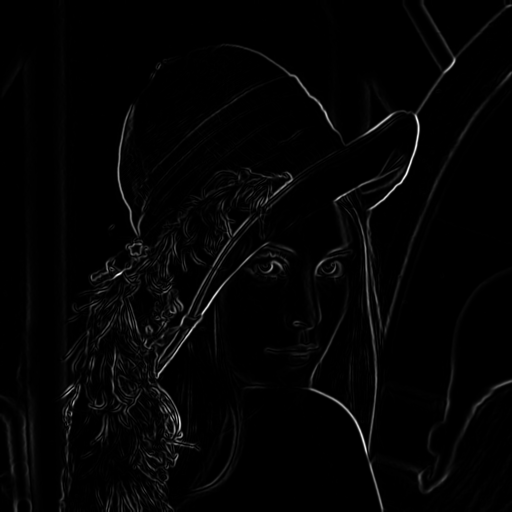
\includegraphics[height=11em]{{{Images/lena/lena_GL_0.1}}} & 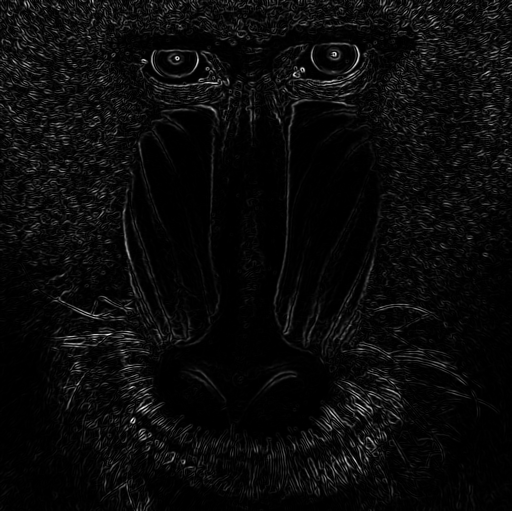
\includegraphics[height=11em]{{{Images/mandrill/mandrill_GL_0.1}}} &  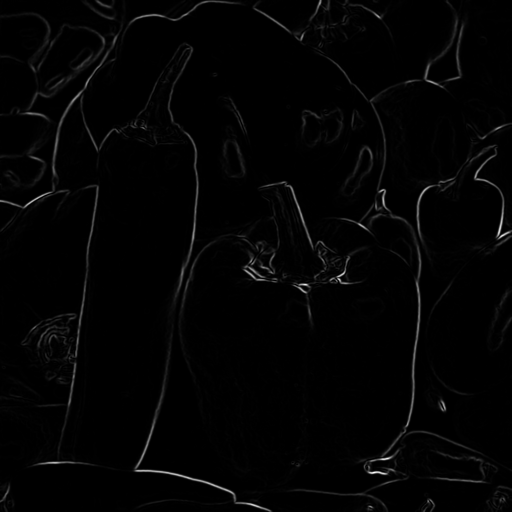
\includegraphics[height=11em]{{{Images/peppers/peppers_GL_0.1}}}\\
    $t = 1.7$ & 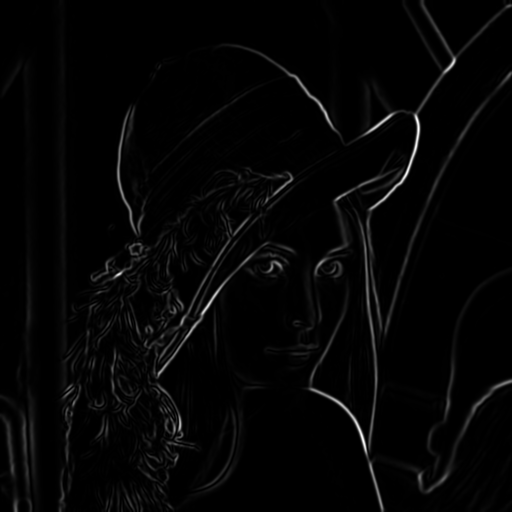
\includegraphics[height=11em]{{{Images/lena/lena_GL_1.7}}} & 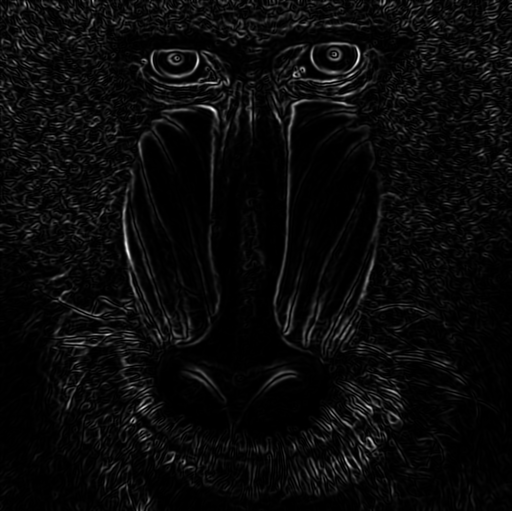
\includegraphics[height=11em]{{{Images/mandrill/mandrill_GL_1.7}}} & 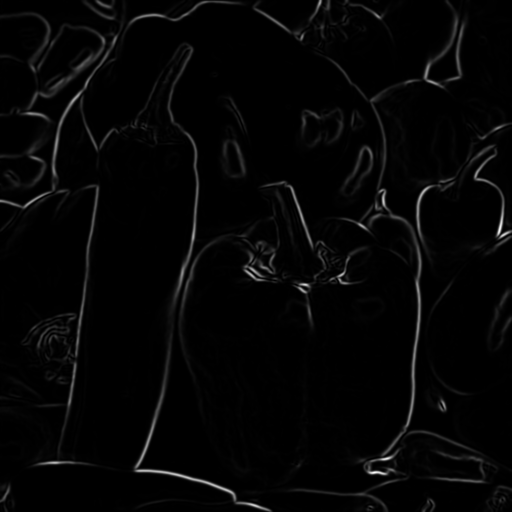
\includegraphics[height=11em]{{{Images/peppers/peppers_GL_1.7}}}\\
    $t = 18.7$ & 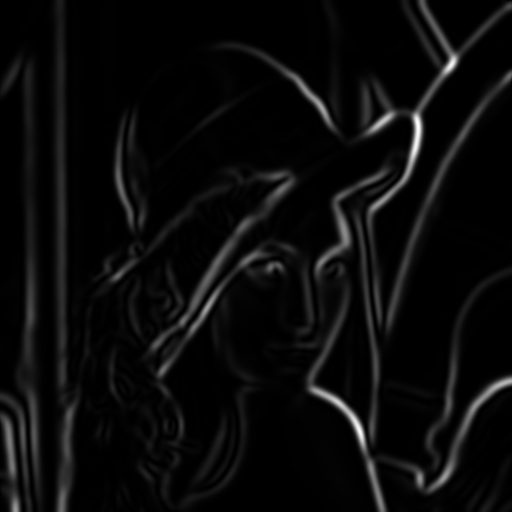
\includegraphics[height=11em]{{{Images/lena/lena_GL_18.7}}} & 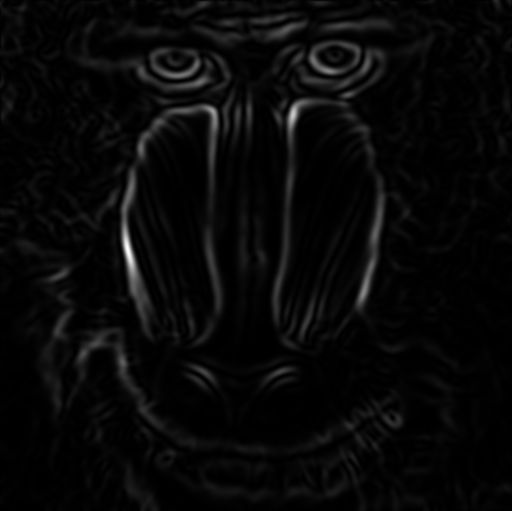
\includegraphics[height=11em]{{{Images/mandrill/mandrill_GL_18.7}}} &  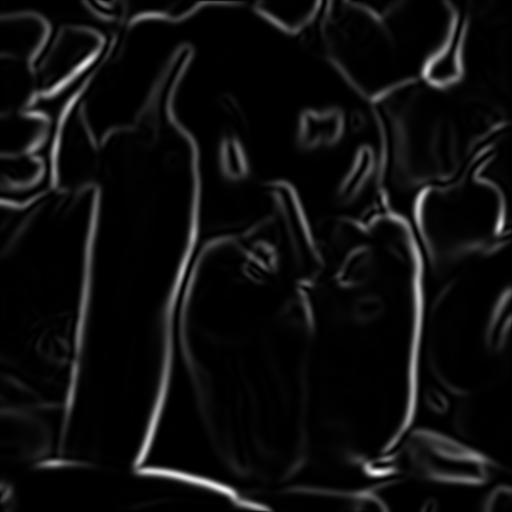
\includegraphics[height=11em]{{{Images/peppers/peppers_GL_18.7}}}\\
    $t = 93.6$ & 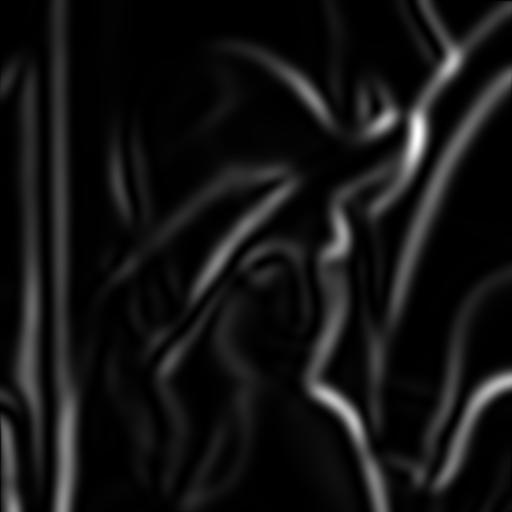
\includegraphics[height=11em]{{{Images/lena/lena_GL_93.6}}} & 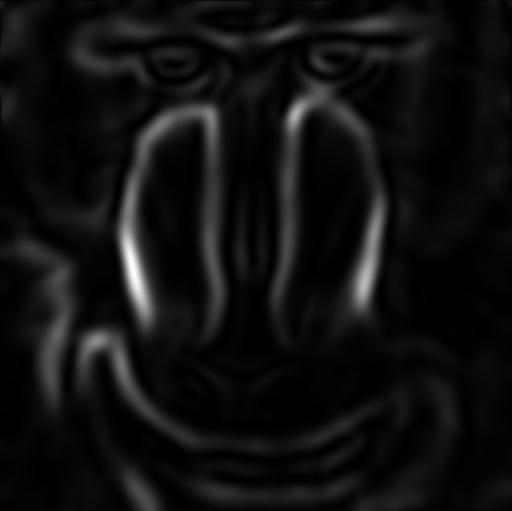
\includegraphics[height=11em]{{{Images/mandrill/mandrill_GL_93.6}}} &  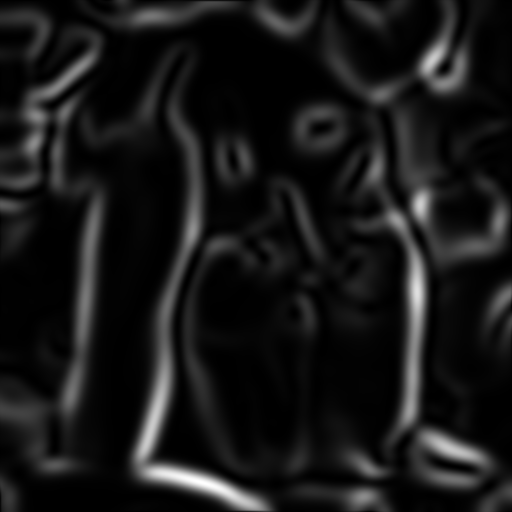
\includegraphics[height=11em]{{{Images/peppers/peppers_GL_93.6}}}\\
    $t = 256.0$ & 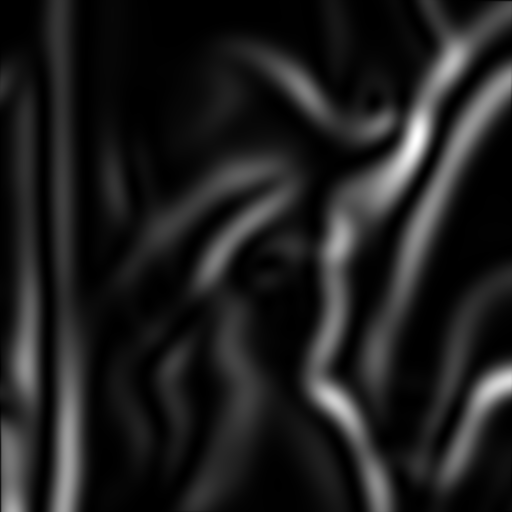
\includegraphics[height=11em]{{{Images/lena/lena_GL_256.0}}} & 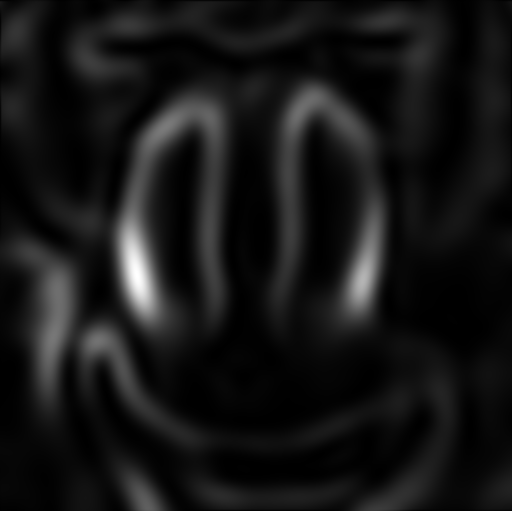
\includegraphics[height=11em]{{{Images/mandrill/mandrill_GL_256.0}}} &  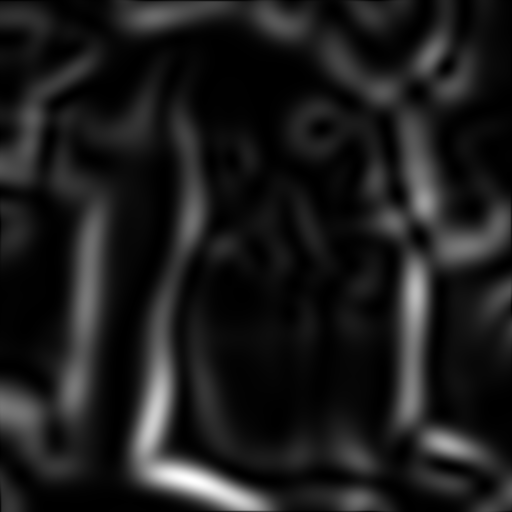
\includegraphics[height=11em]{{{Images/peppers/peppers_GL_256.0}}}\\
    \bottomrule
\end{tabu}
\end{table}
\begin{table}[H]
  \caption{First scale derivative of gradient magnitude}
  \label{t_tgma}
  \centering
  \tabulinesep=0.1em
  \begin{tabu}to \textwidth{cX[c,m]X[c,m]X[c,m]}
    \toprule
    & Lena & Mandrill & Peppers\\
    \midrule
    $t = 0.1$ & 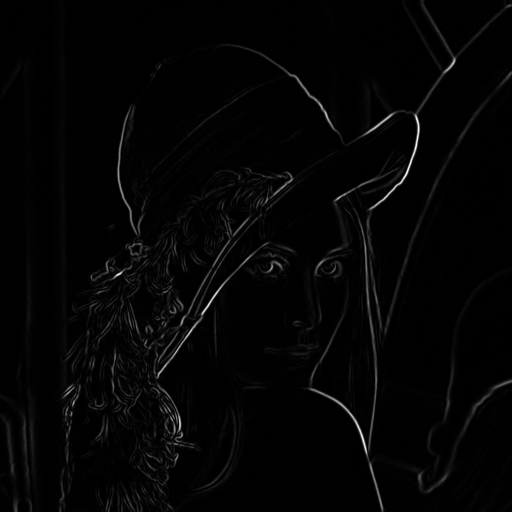
\includegraphics[height=11em]{{{Images/lena/lena_GLt_0.1}}} & 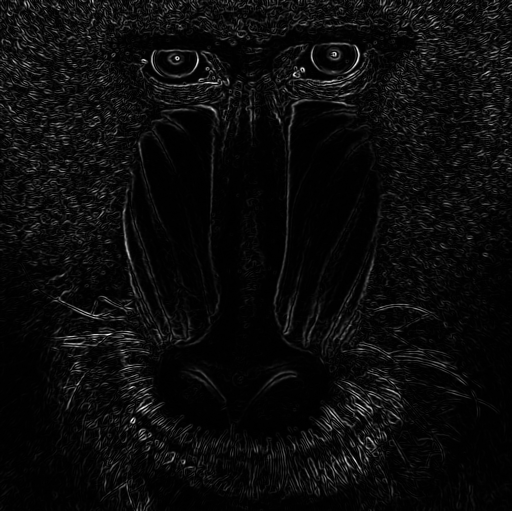
\includegraphics[height=11em]{{{Images/mandrill/mandrill_GLt_0.1}}} &  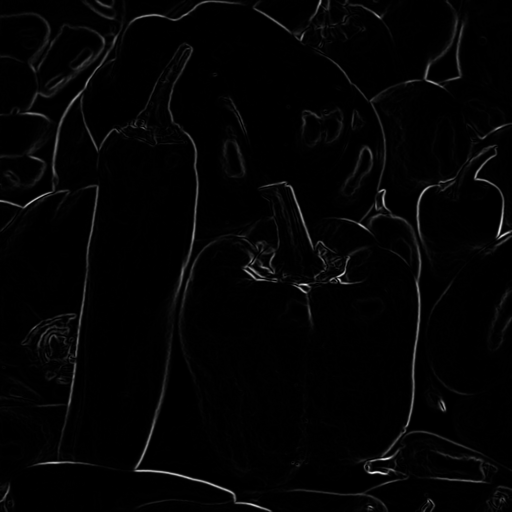
\includegraphics[height=11em]{{{Images/peppers/peppers_GLt_0.1}}}\\
    $t = 1.7$ & 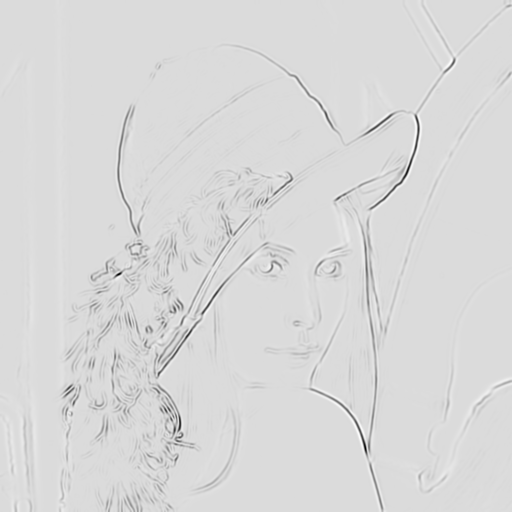
\includegraphics[height=11em]{{{Images/lena/lena_GLt_1.7}}} & 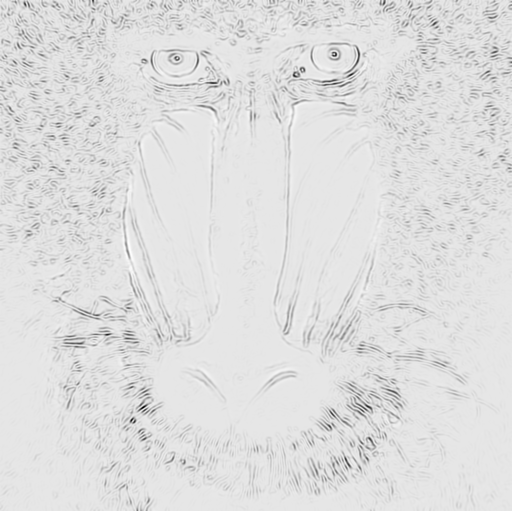
\includegraphics[height=11em]{{{Images/mandrill/mandrill_GLt_1.7}}} & 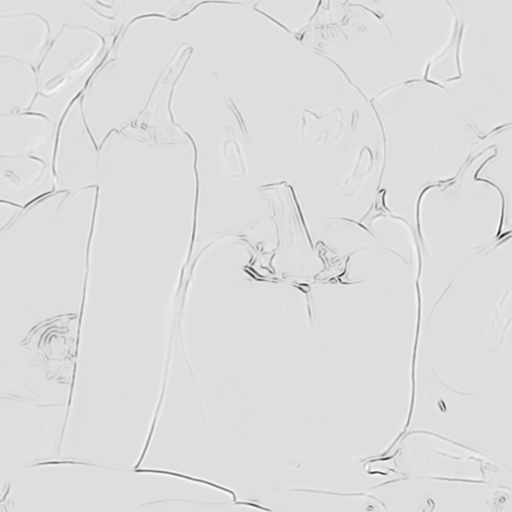
\includegraphics[height=11em]{{{Images/peppers/peppers_GLt_1.7}}}\\
    $t = 18.7$ & 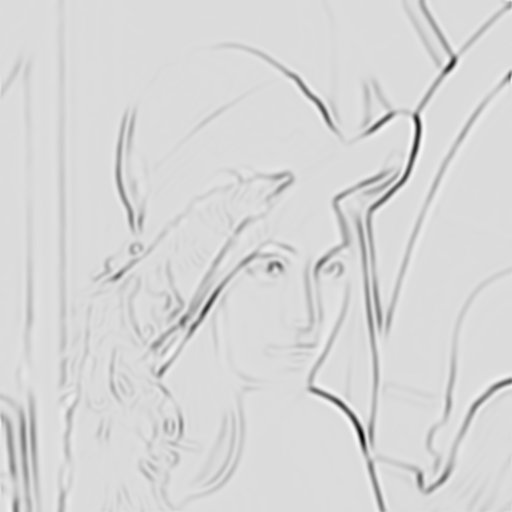
\includegraphics[height=11em]{{{Images/lena/lena_GLt_18.7}}} & 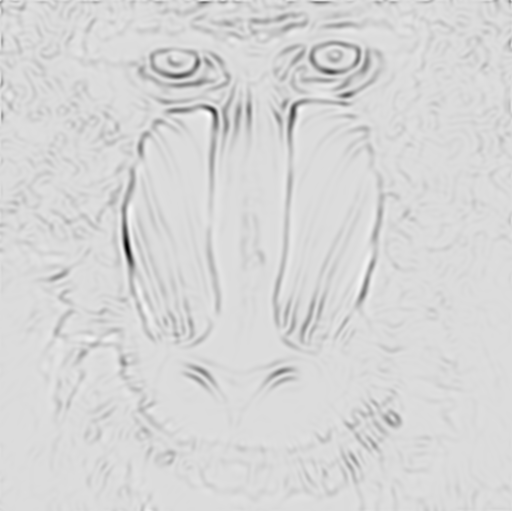
\includegraphics[height=11em]{{{Images/mandrill/mandrill_GLt_18.7}}} &  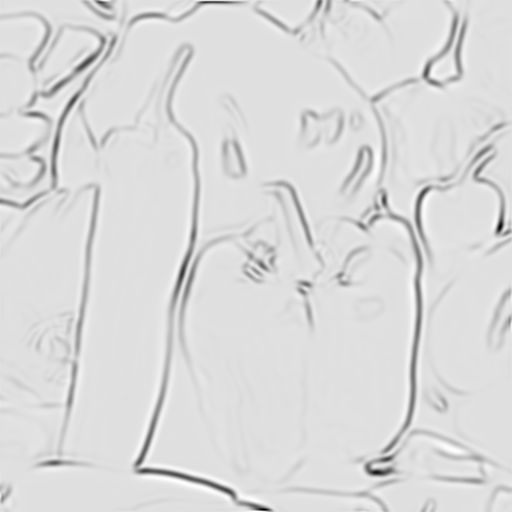
\includegraphics[height=11em]{{{Images/peppers/peppers_GLt_18.7}}}\\
    $t = 93.6$ & 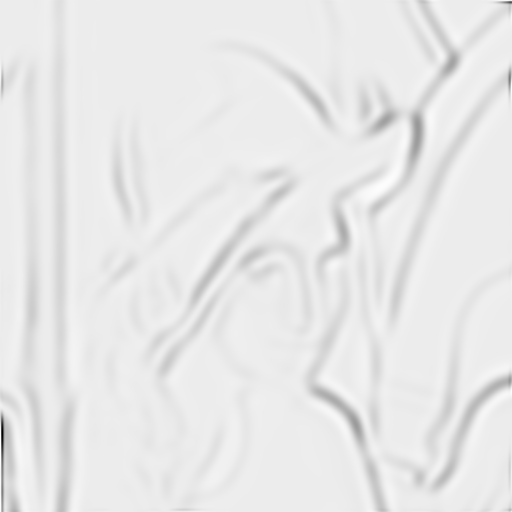
\includegraphics[height=11em]{{{Images/lena/lena_GLt_93.6}}} & 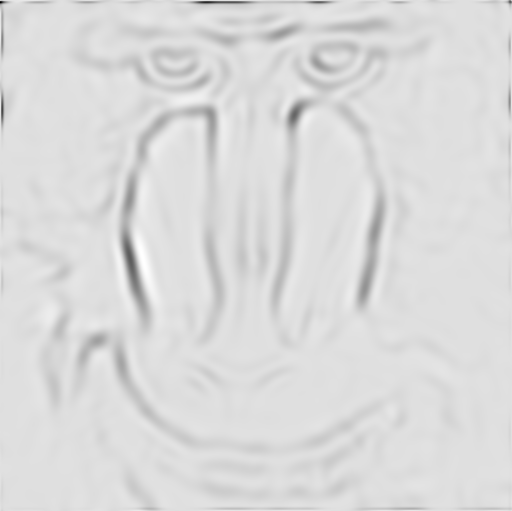
\includegraphics[height=11em]{{{Images/mandrill/mandrill_GLt_93.6}}} &  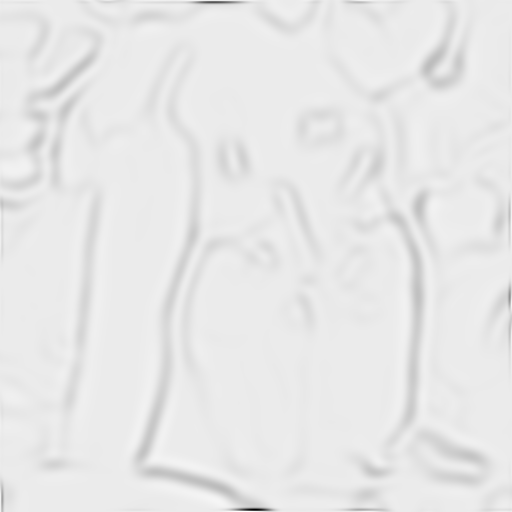
\includegraphics[height=11em]{{{Images/peppers/peppers_GLt_93.6}}}\\
    $t = 256.0$ & 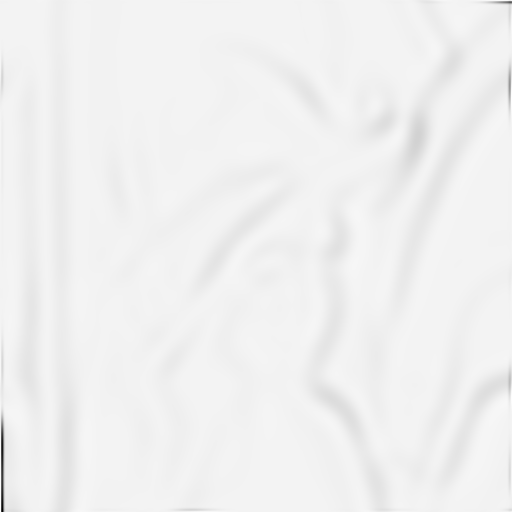
\includegraphics[height=11em]{{{Images/lena/lena_GLt_256.0}}} & 
\includegraphics[height=11em]{{{Images/mandrill/mandrill_GLt_256.0}}} &  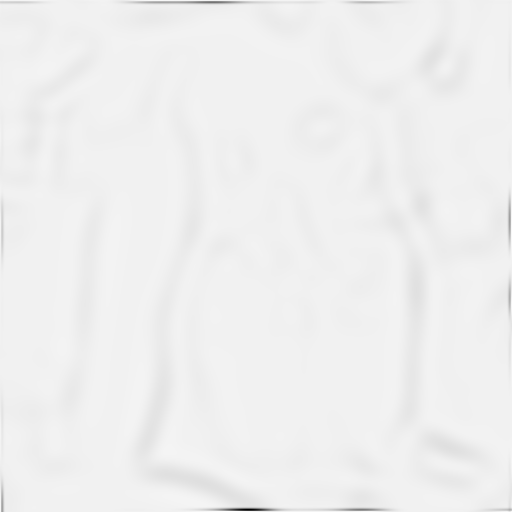
\includegraphics[height=11em]{{{Images/peppers/peppers_GLt_256.0}}}\\
    \bottomrule
\end{tabu}
\end{table}
\begin{table}[H]
  \caption{Second scale derivative of the gradient magnitude}
  \label{t_ttgma}
  \centering
  \tabulinesep=0.1em
  \begin{tabu}to \textwidth{cX[c,m]X[c,m]X[c,m]}
    \toprule
    & Lena & Mandrill & Peppers\\
    \midrule
    $t = 0.1$ & 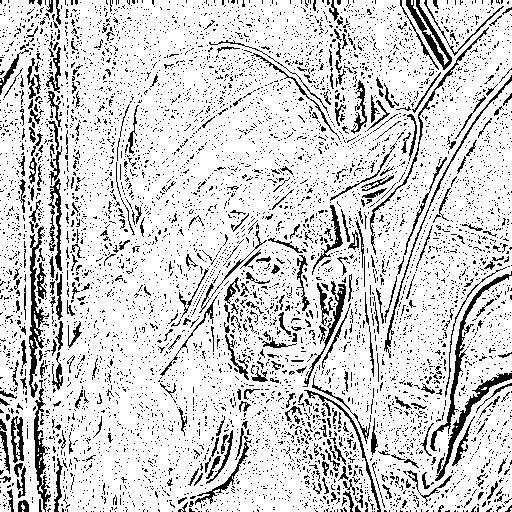
\includegraphics[height=11em]{{{Images/lena/lena_GLtt_0.1}}} & 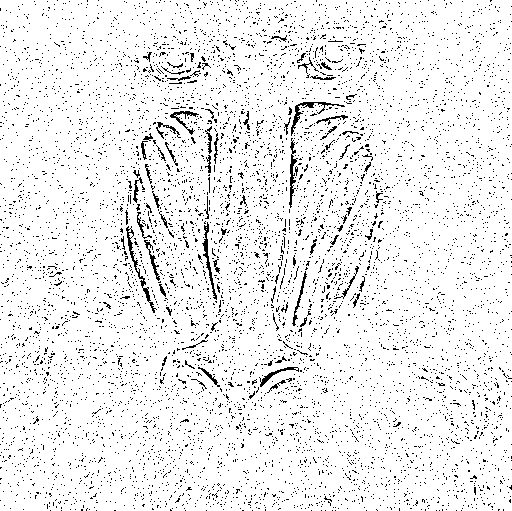
\includegraphics[height=11em]{{{Images/mandrill/mandrill_GLtt_0.1}}} &  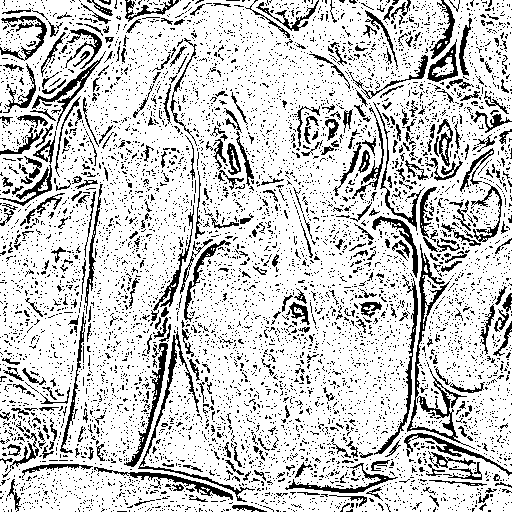
\includegraphics[height=11em]{{{Images/peppers/peppers_GLtt_0.1}}}\\
    $t = 1.7$ & 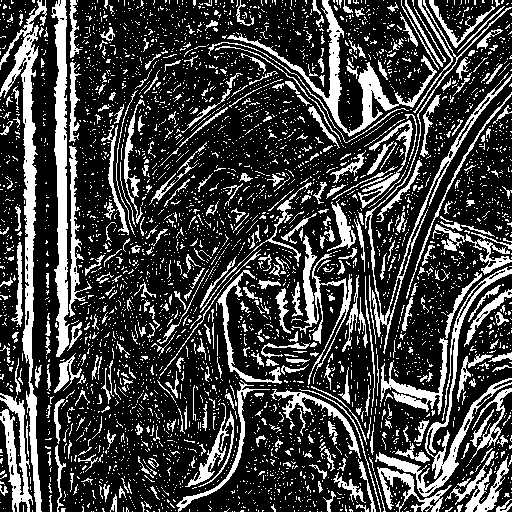
\includegraphics[height=11em]{{{Images/lena/lena_GLtt_1.7}}} & 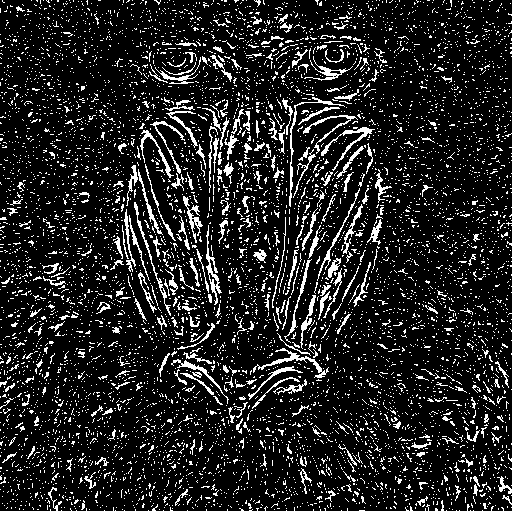
\includegraphics[height=11em]{{{Images/mandrill/mandrill_GLtt_1.7}}} & 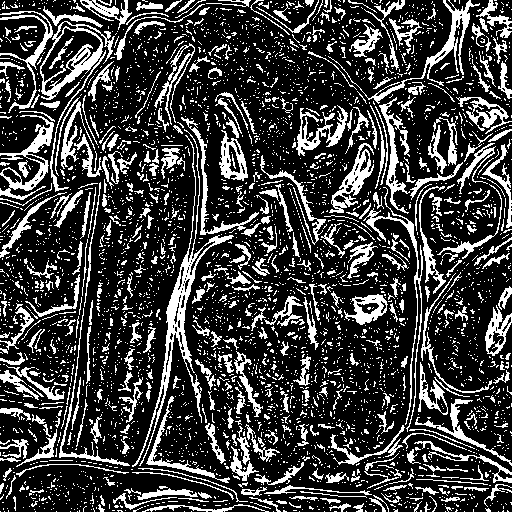
\includegraphics[height=11em]{{{Images/peppers/peppers_GLtt_1.7}}}\\
    $t = 18.7$ & 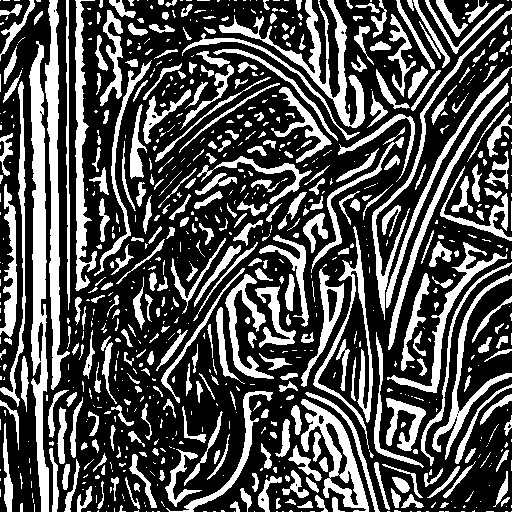
\includegraphics[height=11em]{{{Images/lena/lena_GLtt_18.7}}} & 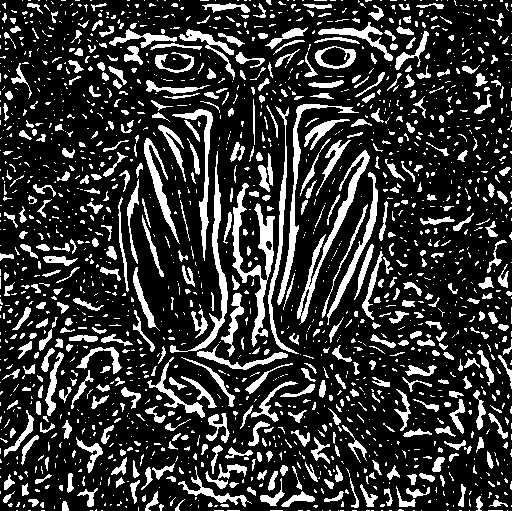
\includegraphics[height=11em]{{{Images/mandrill/mandrill_GLtt_18.7}}} &  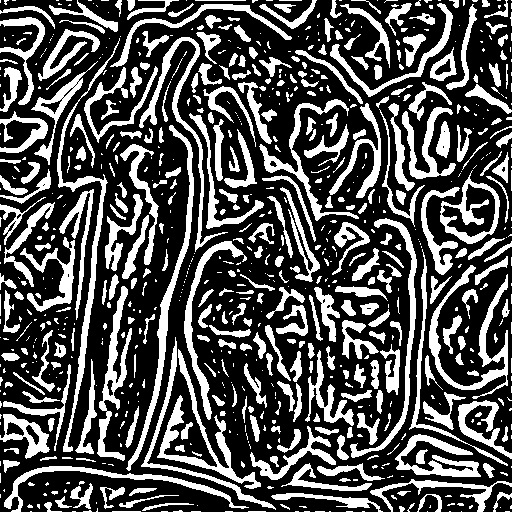
\includegraphics[height=11em]{{{Images/peppers/peppers_GLtt_18.7}}}\\
    $t = 93.6$ & 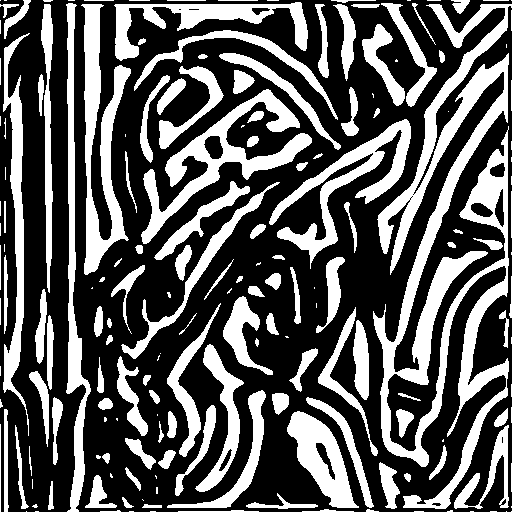
\includegraphics[height=11em]{{{Images/lena/lena_GLtt_93.6}}} & 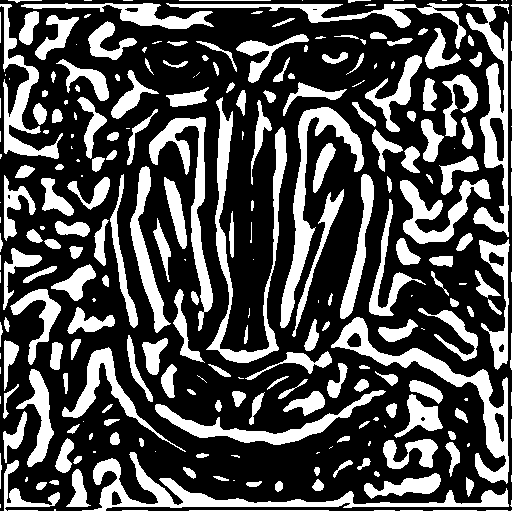
\includegraphics[height=11em]{{{Images/mandrill/mandrill_GLtt_93.6}}} &  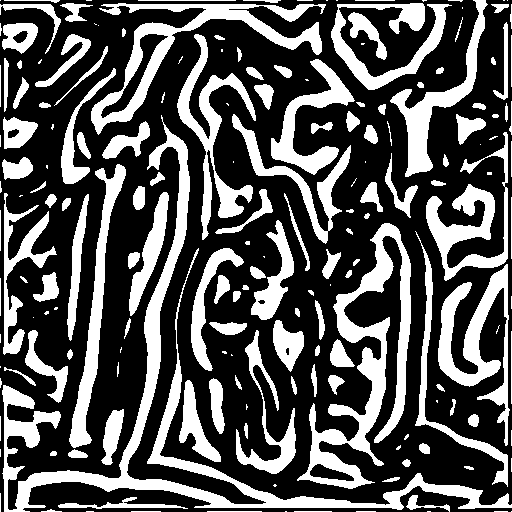
\includegraphics[height=11em]{{{Images/peppers/peppers_GLtt_93.6}}}\\
    $t = 256.0$ & 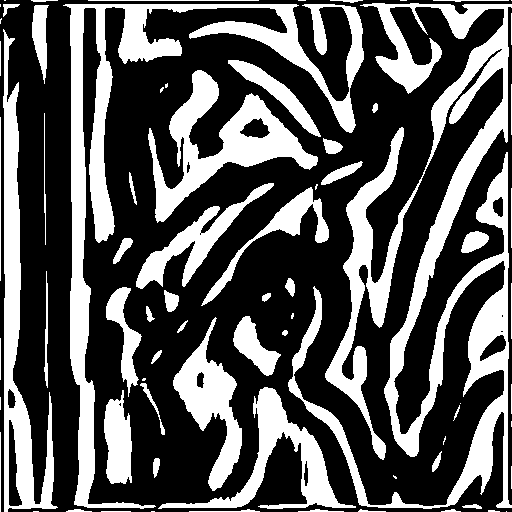
\includegraphics[height=11em]{{{Images/lena/lena_GLtt_256.0}}} & 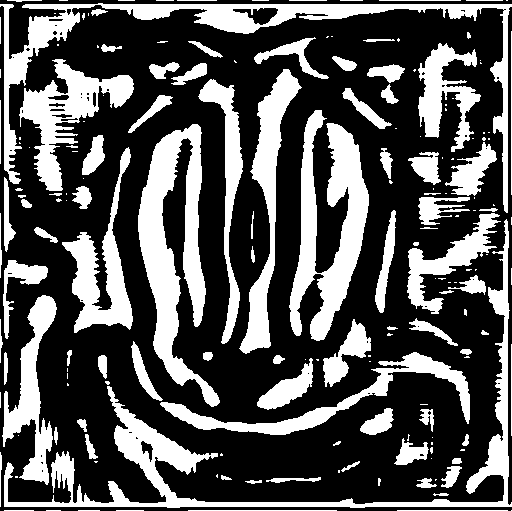
\includegraphics[height=11em]{{{Images/mandrill/mandrill_GLtt_256.0}}} &  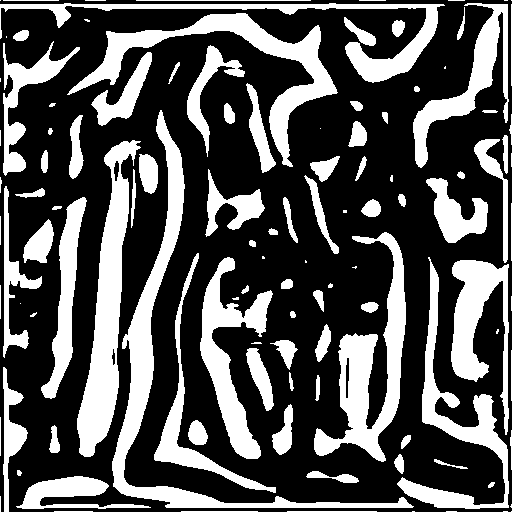
\includegraphics[height=11em]{{{Images/peppers/peppers_GLtt_256.0}}}\\
    \bottomrule
\end{tabu}
\end{table}
\begin{table}[H]
  \caption{Maxima of scale space in the $v$ direction}
  \label{t_v}
  \centering
  \tabulinesep=0.1em
  \begin{tabu}to \textwidth{cX[c,m]X[c,m]X[c,m]}
    \toprule
    & Lena & Mandrill & Peppers\\
    \midrule
    $t = 0.1$ & 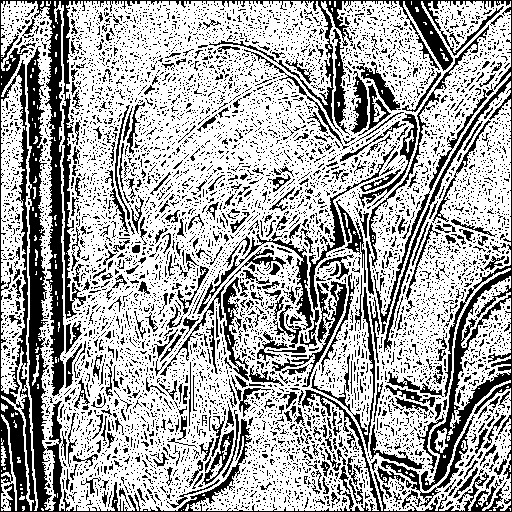
\includegraphics[height=11em]{{{Images/lena/lena_Lv_maxima_0.1}}} & 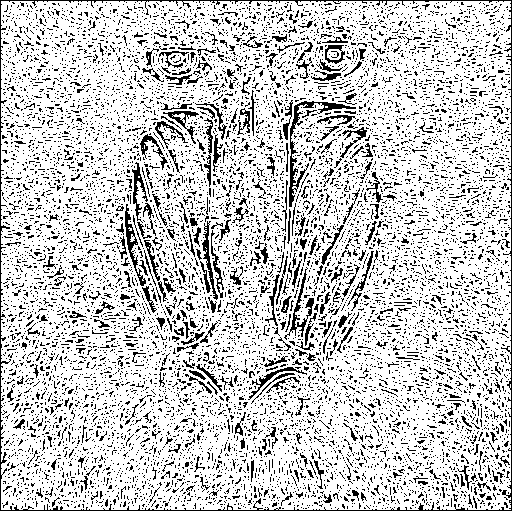
\includegraphics[height=11em]{{{Images/mandrill/mandrill_Lv_maxima_0.1}}} &  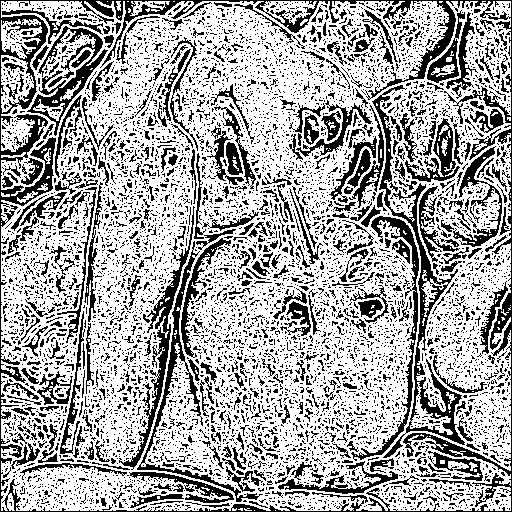
\includegraphics[height=11em]{{{Images/peppers/peppers_Lv_maxima_0.1}}}\\
    $t = 1.7$ & 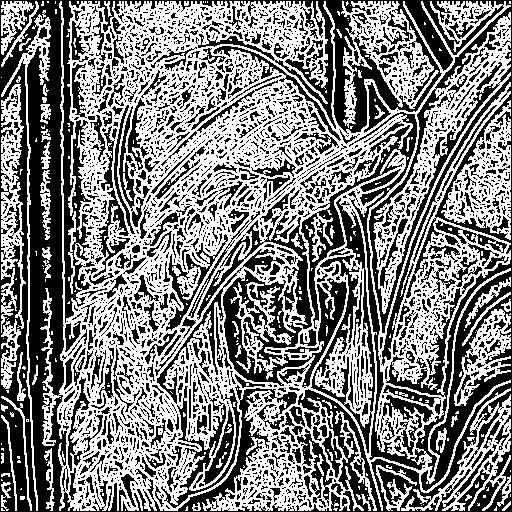
\includegraphics[height=11em]{{{Images/lena/lena_Lv_maxima_1.7}}} & 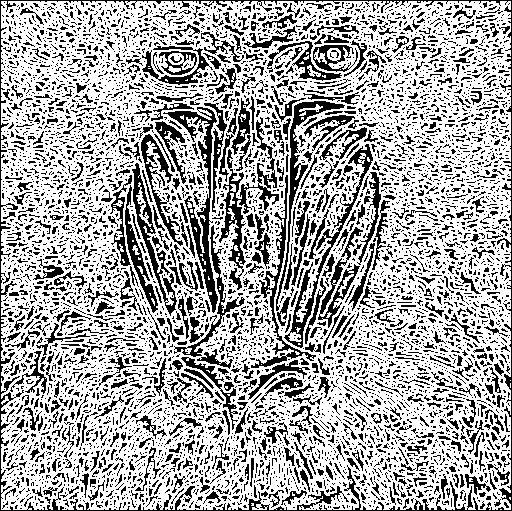
\includegraphics[height=11em]{{{Images/mandrill/mandrill_Lv_maxima_1.7}}} & \includegraphics[height=11em]{{{Images/peppers/peppers_Lv_maxima_1.7}}}\\
    $t = 18.7$ & \includegraphics[height=11em]{{{Images/lena/lena_Lv_maxima_18.7}}} & \includegraphics[height=11em]{{{Images/mandrill/mandrill_Lv_maxima_18.7}}} &  \includegraphics[height=11em]{{{Images/peppers/peppers_Lv_maxima_18.7}}}\\
    $t = 93.6$ & \includegraphics[height=11em]{{{Images/lena/lena_Lv_maxima_93.6}}} & \includegraphics[height=11em]{{{Images/mandrill/mandrill_Lv_maxima_93.6}}} &  \includegraphics[height=11em]{{{Images/peppers/peppers_Lv_maxima_93.6}}}\\
    $t = 256.0$ & \includegraphics[height=11em]{{{Images/lena/lena_Lv_maxima_256.0}}} & \includegraphics[height=11em]{{{Images/mandrill/mandrill_Lv_maxima_256.0}}} &  \includegraphics[height=11em]{{{Images/peppers/peppers_Lv_maxima_256.0}}}\\
    \bottomrule
\end{tabu}
\end{table}
\begin{table}[H]
  \caption{The second derivative of the scale space with respect to the $v$ direction}
  \label{t_vv}
  \centering
  \tabulinesep=0.1em
  \begin{tabu}to \textwidth{cX[c,m]X[c,m]X[c,m]}
    \toprule
    & Lena & Mandrill & Peppers\\
    \midrule
    $t = 0.1$ & \includegraphics[height=11em]{{{Images/lena/lena_Lvv_0.1}}} & \includegraphics[height=11em]{{{Images/mandrill/mandrill_Lvv_0.1}}} &  \includegraphics[height=11em]{{{Images/peppers/peppers_Lvv_0.1}}}\\
    $t = 1.7$ & \includegraphics[height=11em]{{{Images/lena/lena_Lvv_1.7}}} & \includegraphics[height=11em]{{{Images/mandrill/mandrill_Lvv_1.7}}} & \includegraphics[height=11em]{{{Images/peppers/peppers_Lvv_1.7}}}\\
    $t = 18.7$ & \includegraphics[height=11em]{{{Images/lena/lena_Lvv_18.7}}} & \includegraphics[height=11em]{{{Images/mandrill/mandrill_Lvv_18.7}}} &  \includegraphics[height=11em]{{{Images/peppers/peppers_Lvv_18.7}}}\\
    $t = 93.6$ & \includegraphics[height=11em]{{{Images/lena/lena_Lvv_93.6}}} & \includegraphics[height=11em]{{{Images/mandrill/mandrill_Lvv_93.6}}} &  \includegraphics[height=11em]{{{Images/peppers/peppers_Lvv_93.6}}}\\
    $t = 256.0$ & \includegraphics[height=11em]{{{Images/lena/lena_Lvv_256.0}}} & \includegraphics[height=11em]{{{Images/mandrill/mandrill_Lvv_256.0}}} &  \includegraphics[height=11em]{{{Images/peppers/peppers_Lvv_256.0}}}\\
    \bottomrule
\end{tabu}
\end{table}
\begin{table}[H]
  \caption{The third derivative of the scale space with respect to the $v$ direction}
  \label{t_vvv}
  \centering
  \tabulinesep=0.1em
  \begin{tabu}to \textwidth{cX[c,m]X[c,m]X[c,m]}
    \toprule
    & Lena & Mandrill & Peppers\\
    \midrule
    $t = 0.1$ & \includegraphics[height=11em]{{{Images/lena/lena_Lvvv_0.1}}} & \includegraphics[height=11em]{{{Images/mandrill/mandrill_Lvvv_0.1}}} &  \includegraphics[height=11em]{{{Images/peppers/peppers_Lvvv_0.1}}}\\
    $t = 1.7$ & \includegraphics[height=11em]{{{Images/lena/lena_Lvvv_1.7}}} & \includegraphics[height=11em]{{{Images/mandrill/mandrill_Lvvv_1.7}}} & \includegraphics[height=11em]{{{Images/peppers/peppers_Lvvv_1.7}}}\\
    $t = 18.7$ & \includegraphics[height=11em]{{{Images/lena/lena_Lvvv_18.7}}} & \includegraphics[height=11em]{{{Images/mandrill/mandrill_Lvvv_18.7}}} &  \includegraphics[height=11em]{{{Images/peppers/peppers_Lvvv_18.7}}}\\
    $t = 93.6$ & \includegraphics[height=11em]{{{Images/lena/lena_Lvvv_93.6}}} & \includegraphics[height=11em]{{{Images/mandrill/mandrill_Lvvv_93.6}}} &  \includegraphics[height=11em]{{{Images/peppers/peppers_Lvvv_93.6}}}\\
    $t = 256.0$ & \includegraphics[height=11em]{{{Images/lena/lena_Lvvv_256.0}}} & \includegraphics[height=11em]{{{Images/mandrill/mandrill_Lvvv_256.0}}} &  \includegraphics[height=11em]{{{Images/peppers/peppers_Lvvv_256.0}}}\\
    \bottomrule
\end{tabu}
\end{table}
% \lstinputlisting[caption={edge\_detect.jl},label=edge_detect,frame=none]{edge_detect.jl}

\bibliography{bibliography}{}
\bibliographystyle{plain}

\end{document}
